\documentclass{article}
\pdfpagewidth=8.5in
\pdfpageheight=11in

\usepackage{ijcai26}


\usepackage{times}
\usepackage{soul}
\usepackage{url}
\usepackage[hidelinks]{hyperref}
\usepackage[utf8]{inputenc}
\usepackage[small]{caption}
\usepackage{graphicx}


\usepackage{amsmath}
\usepackage{amsthm}
\usepackage{amssymb}
\usepackage{amsfonts}
\usepackage{bm}


\usepackage{booktabs}
\usepackage{multirow}
\usepackage{threeparttable}
\usepackage{algorithm}
\usepackage{algorithmic}
\usepackage{booktabs}
\usepackage{longtable}
\usepackage{tabularx}
\usepackage{makecell}
\usepackage{geometry} % 可选，如果需要微调页边距


\usepackage{subfig} 
\usepackage[table]{xcolor}
\usepackage{placeins}


\usepackage{xcolor}
\usepackage[switch]{lineno}
\linenumbers

\pdfinfo{
/TemplateVersion (IJCAI.2026.0)
}


\begin{document}

\onecolumn % 切换单栏

% --- 手动写一个居中的大标题 ---
\begin{center}
    {\LARGE \textbf{Appendix for Stage-Aware Multi-Task Reinforcement Learning for Sparse Reward Tasks}}
\end{center}
\vspace{1em} % 增加一点垂直间距

% --- 正文开始 ---
\section{Appendix}




\begin{table}[!htbp]
\centering
\footnotesize % 使用 small 字体，比 footnotesize 大一点，但比 normal 小，适合宽表
\setlength{\tabcolsep}{2pt} % 适度减小列间距
\renewcommand{\arraystretch}{1.4} % 适度增加行高，提升公式可读性

\begin{threeparttable}
\caption{\textbf{Formal Definitions of Action Primitives and Reward Structures.}
We define the spatial predicate $\texttt{At}(A, B) \iff d(A, B) \le \delta$, where $d(x,y) = \|x-y\|_2$ denotes the Euclidean distance.
We define the spatial predicate $\texttt{Success}(s_t, a_t, s_{t+1}) \iff (\Delta s_{\text{real}} \cdot a_t > 0) \land (\| \Delta s_{\text{real}} \| > \eta \| a_t \|)$.
Specifically, there are two testing modes: sparse reward and dense reward mode based on reward machine.}
\label{tab:action_formalism}

\begin{tabular}{l l l l}
\toprule
\textbf{Primitive}  & \textbf{Precondition} & \textbf{Sparse Mode} ($r_{sparse}$) & \textbf{Dense Mode} ($r_{dense}$) \\
\midrule

% Reach
\texttt{Reach}($A$) & 
$\emptyset$  & 
$\begin{cases} 
r^{\text{goal}}=1, & \text{if } d(H, A) \le \delta_{reach} \\ 
r^{\text{active}}= NA, & \text{otherwise}  \\ 
r^{\text{guide}}= NA, & \text{otherwise} 
\end{cases}$ & 
$\begin{cases} 
r^{\text{goal}}=1, & \text{if } d(H, A) \le \delta_{reach} \\ 
r^{\text{active}}= NA,  & \text{if } \text{Precond.}  \\ 
r^{\text{guide}}= {\lambda_1 d_{r}(H,A)},  & \text{if } \text{Precond.} 
\end{cases}$ \\


\addlinespace[4pt]

% Move
\texttt{Move}($A, B$) & 
$d(H, A) \le \delta_{reach}$ & 
$\begin{cases} 
r^{\text{goal}}=1, & \text{if } d(A, B) \le \delta_{reach} \\ 
r^{\text{active}}= \lambda_1 \mathbb{I}(\texttt{Succ}),  & \text{if } d(H, A) \le \delta_{reach} \\ 
r^{\text{guide}}= NA, & \text{otherwise} 
\end{cases}$ & 
$\begin{cases} 
r^{\text{goal}}=1, & \text{if } d(A, B) \le \delta_{reach} \\ 
r^{\text{active}}=\lambda_1 d_r(H, A),  & \text{if } \text{Precond.}  \\ 
r^{\text{guide}}=  {\lambda_2 d_r(A, B)}  & \text{if } \text{Precond.}  
\end{cases}$ \\

\addlinespace[4pt]

% Press
\texttt{Press}($A, B$) & 
$d(H, A) \le \delta_{reach}$ & 
$\begin{cases} 
r^{\text{goal}}=1, & \text{if } d(A, B) \le \delta_{press} \\ 
r^{\text{active}}= \lambda_1 ,  & \text{if } d(H, A) \le \delta_{reach} \\ 
r^{\text{guide}}= NA, & \text{otherwise} 
\end{cases}$ & 
$\begin{cases} 
r^{\text{goal}}=1, & \text{if } d(A, B) \le \delta_{press} \\ 
r^{\text{active}}=\lambda_1 d_r(H, A),  & \text{if } \text{Precond.}  \\ 
r^{\text{guide}}=  {\lambda_3 d_r(A, B)}  & \text{if } \text{Precond.} 
\end{cases}$ \\

\addlinespace[4pt]

% Turn
\texttt{Turn}($A, B$) & 
$d(H, A) \le \delta_{reach}$ & 
$\begin{cases} 
r^{\text{goal}}=1, & \text{if } d(A, B) \le \delta_{turn} \\ 
r^{\text{active}}=\lambda_1  , & \text{if } d(H, A) \le \delta_{reach} \\ 
r^{\text{guide}}= NA, & \text{otherwise} 
\end{cases}$ & 
$\begin{cases} 
r^{\text{goal}}=1, & \text{if } d(A, B) \le \delta_{turn} \\ 
r^{\text{active}}=\lambda_1 d_r(H, A),  & \text{if } \text{Precond.} \\ 
r^{\text{guide}}=  {\lambda_4 d_r(A, B)}  & \text{if } \text{Precond.} 
\end{cases}$ \\


% Manipulate
\texttt{Manip.}($B, C$) & 
\makecell{$d(H, A) \le \delta_{reach}$ \\ $d(A, B) \le \delta_{reach}$} & 
% Sparse Mode
$\begin{cases} 
r^{\text{goal}}=1, & \text{if } d(B, C) \le \delta_{reach} \\ 
r^{\text{active}}=(\lambda_1 + \lambda_2)\mathbb{I}(\texttt{Succ}), & \text{if } \text{Precond.} \\ 
r^{\text{guide}}= NA, & \text{otherwise} 
\end{cases}$ & 
% Dense Mode
$\begin{cases} 
r^{\text{goal}}=1, & \text{if } d(B, C) \le \delta_{reach} \\ 
r^{\text{active}}= \begin{aligned} \lambda_1 d_r(H, A) \\  + \lambda_2 d_r(A, B) \end{aligned}, & \text{if } \text{Precond.} \\
r^{\text{guide}}= \lambda_5 d_r(B, C),  & \text{if } \text{Precond.} 
\end{cases}$ \\


\bottomrule
\end{tabular}

\begin{tablenotes}
\footnotesize
\item \textbf{Notation:} ${d_{r}(A,B)=0.5(\exp \left( -\frac{d(A, B)^2}{2\sigma_1^2} \right) + \exp \left( -\frac{d(A, B)^2}{2\sigma_2^2}\right)) },$ $2\sigma_1^2=0.125,2\sigma_2^2=0.001$ %+ (-||A,B||)%
\item \textbf{Parameters:} Distance thresholds are set as $\delta_{reach} =  0.05$, $\delta_{press} = 0.03$, and $\delta_{turn} = 0.02$ . $\lambda_1=\lambda_2=\lambda_5=0.3,\lambda_3=\lambda_4=0.6$
\item \textbf{Notation:} $H$ denotes the end-effector.
\end{tablenotes}
\end{threeparttable}
\end{table}



\textbf{0. Formal Definition of Task Primitives (The Symbolic Basis).}

By definition, we formalize the action primitive for the $j$th stage as a quintuple:
$$p_j \triangleq \left( \mathcal{S}_j, \mathcal{G}_j, r_j^{\text{active}}, r_j^{\text{guide}}, r_j^{\text{goal}} \right)$$
where:

$\mathcal{S}_j \subseteq \mathcal{S} \subset \mathbb{R}^{3K}$
is the state space within which executing $p_j$ is legal.

$\mathcal{G}_j \subset \mathcal{S}$ is the goal set.

$r_j^{\text{active}}: \mathcal{S}_j \times \mathcal{A} \times \mathcal{S} \to [-1, 1]$ is the reward for staying with $p_j$.

$r_j^{\text{guide}}: \mathcal{S}_j \times \mathcal{A} \times \mathcal{S}_j \to [-1, 1]$ is the reward for guiding actions. 

$r_j^{\text{goal}}: \mathcal{S}_j \times \mathcal{A} \times \mathcal{G}_j \to [-1, 1]$ is the reward for accomplishing $p_j$.


\textbf{1. Prim Similarity Calculation}


$$\text{Sim}(p_i, p_j) = 1 - \frac{\int |r_i(s) - r_j(s)| ds}{\int |r_i(s)| ds + \int |r_j(s)| ds}$$

$$V(\delta) = \int_{\mathbb{R}^3} \mathbb{I}(\|x\|_2 \le \delta) \, dx = \frac{4}{3}\pi \delta^3$$

$$E_\Psi(\sigma) = \int_{\mathbb{R}^3} \lambda e^{-\frac{\|x\|^2}{2\sigma^2}} \, dx = \lambda (\sqrt{2\pi}\sigma)^3$$


\texttt{Reach}:  $\|r_{Reach}\| = \underbrace{ \lambda_1 E_{\Psi}}_{r^{\text{guide}}} + \underbrace{V(\delta_{reach})}_{r^{\text{goal}}}$

\texttt{Move}: $\|r_{Move}\| = \underbrace{ \lambda_1 E_{\Psi}}_{r^{\text{active}}} + \underbrace{\lambda_2 E_{\Psi}}_{r^{\text{guide}}} + \underbrace{V(\delta_{reach})}_{r^{\text{goal}}} = 2E_{\Psi} + V(\delta_{reach})$

\texttt{Press}: $\|r_{Press}\| = \lambda_1 E_{\Psi} + \lambda_3 E_{\Psi} +V(\delta_{press})$

\texttt{Turn}: $\|r_{Turn}\| = \lambda_1 E_{\Psi} + \lambda_4 E_{\Psi} + V(\delta_{turn})$

\texttt{Manip.}: $\|r_{Manip.}\| = \lambda_1 E_{\Psi} + \lambda_2 E_{\Psi} + \lambda_5 E_{\Psi} + V(\delta_{reach})$


\begin{table}[htbp]
\centering
\caption{Similarity Matrices of Action Primitives under Dense and Sparse Reward Settings. 
Dense rewards show high transferability (overlap) due to shared potential fields, while sparse rewards show lower similarity due to disjoint goal regions.}
\label{tab:sim_matrices}
\renewcommand{\arraystretch}{1.2}
\setlength{\tabcolsep}{5pt}

\begin{tabular}{l l S S S S S}
\toprule
\textbf{Setting} & \textbf{Primitive} & {\textbf{Reach}} & {\textbf{Move}} & {\textbf{Press}} & {\textbf{Turn}} & {\textbf{Manip}} \\
\midrule

\multirow{5}{*}{\rotatebox{90}{\textbf{Dense}}} 
& Reach & 1.00 & 0.66 & 0.50 & 0.50 & 0.50 \\
& Move  & 0.66 & 1.00 & 0.80 & 0.79 & 0.80 \\
& Press & 0.50 & 0.80 & 1.00 & 0.99 & 0.66 \\
& Turn  & 0.50 & 0.79 & 0.99 & 1.00 & 0.66 \\
& Manip & 0.50 & 0.80 & 0.66 & 0.66 & 1.00 \\
\midrule

\multirow{5}{*}{\rotatebox{90}{\textbf{Sparse}}} 
& Reach & 1.00 & 0.26 & 0.39 & 0.43 & 0.00 \\
& Move  & 0.26 & 1.00 & 0.57 & 0.43 & 0.23 \\
& Press & 0.39 & 0.57 & 1.00 & 0.82 & 0.06 \\
& Turn  & 0.43 & 0.43 & 0.82 & 1.00 & 0.02 \\
& Manip & 0.00 & 0.23 & 0.06 & 0.02 & 1.00 \\

\bottomrule
\end{tabular}
\end{table}


%A constraint-based method for solving  sequential manipulation planning problems论文采用分层架构，上层是符号规划（Symbolic Planning），下层是几何约束求解。动作原语（如 Pick, Move）首先作为符号算子被检索，必须满足符号前置条件。该论文前置约束满足输出的是0，1，不同前置得到的是不同原语。目前我们前提条件作为约束条件。不同约束视为不在同一前置条件下的原语，因此第一项先验相似性为0，1函数。

%An Object-Oriented Representation for Efficient Reinforcement Learning 论文证明，如果两个状态在“对象属性”和“相互关系”上是一致的（即便对象 ID 不同），Agent 学到的效果是可以泛化的（迷宫环境）。第二项奖励函数变量的 Jaccard 相似性可以计算得到在对应奖励函数下，动作原语和哪些变量相关，输出范围为[0,1]。


%第一项确保前提条件一致，基于动作原语定义域S进行相似性度量，输出0，1值作为相似性。第二项计算得到对应奖励函数变量是否相关，使用Jaccard计算原语奖励函数变量相似性。第三项针对目标域的重叠进行计算相似性，从动作原语目标G上进行区分。


\textbf{2.0. Why use data?}

Symbolic isomorphism - different dynamics: 

Although the same primitive instances under different tasks (e.g., $\texttt{Move}(A, B)$ for Task A and $\texttt{Move}(A', B')$ for Task B) share the same reward function template $r(s, a) = \mathbb{I}(d(A, B) \le \delta) - d(A, B)$, the final output policy of their control policy $\pi$ is constrained by the specific geometric layout of the task environment.

Space - Manifold: 

The legal state space $\mathcal{S}_j$ in the primitive definition is a static geometric region (defined by preconditions such as $d(H, A) \le \delta_{reach}$, which is equivalent to $\mathcal{S}$ after fulfilling the preconditions).
However, task similarity is essentially behavioral similarity. Trajectories $\tau$ do not fill the entire $\mathcal{S}_j$, but are distributed across a manifold within $\mathcal{S}_j$. 
Directly calculating the geometric overlap between two high-dimensional nominal spaces $\mathcal{S}_i$ and $\mathcal{S}_j$ not only ignores the actual distribution of the policy within that space but is also extremely sensitive to changes in the absolute coordinate system.
Therefore, we map the primitives to a trajectory distribution in the latent space, aiming to compare the similarity between these two effective manifolds. This elevates the data-driven metric from the instance level to the task-policy level. Unlike the static symbolic template (Prior) which defines the nominal intent, this manifold representation captures the actual geometric constraints of the task, ensuring both metrics operate at the same task-abstraction granularity but cover different aspects.

\textbf{2.1. Data Structure: Stage-wise Trajectory Manifold}

Define the experience dataset $\mathcal{D}$ as a hierarchical trajectory library, jointly indexed by the task index $i \in \{1, \dots, N\}$ and the stage index $k \in \{1, \dots, n\}$.

For any specific primitive instance (i.e., the $k$-th stage of task $T^{(i)}$), we maintain a set of high-value trajectories
$\boldsymbol{\tau}^{(i)}_k$: 

$$\mathcal{D} = \left\{ \boldsymbol{\tau}^{(i)}_k \mid i \in [1, N], k \in [1, n] \right\}$$

Where, a single trajectory $\tau \in \boldsymbol{\tau}^{(i)}_k$ is defined as a state-action sequence: $$\tau = \langle (s_0, a_0, r_0), (s_1, a_1, r_1), \dots, (s_L, a_L, r_L) \rangle$$

Data Constraints: 
To ensure that $\tau$ can represent the primitive's policy $\pi$ The stored data, based on behavioral characteristics (rather than exploratory noise), satisfies the following filtering criteria (corresponding to the Top-K logic in the code): 
Optimality: $\tau \in \boldsymbol{\tau}^{(i)}_k$ rank in the Top-K of the historical replay pool if and only if its cumulative reward $R(\tau) = \sum r_t$ is in the Top-K.

Completion: The sequence length $L$ satisfies $L_{min} \leq L \leq L_{max}$, ensuring that it contains complete stage execution semantics.


\textbf{2.2. Data Similarity Calculation}

Directly comparing the original trajectories $\tau$ is susceptible to interference from absolute coordinates.

To extract pure policy behavior features, we define a normalization transformation $\Psi$, which explicitly utilizes the semantic information (state space $\mathcal{S}_j$ and target set $\mathcal{G}_j$) defined by primitives in $p_j$.

For the state $s_t \in \mathcal{S}$ at any time $t$, according to the parameter definition of $p_j$, we extract the set of absolute coordinates $\mathbf{X}_t$ of Task $i$ key entities $e^{(i)}$: 
$$\mathbf{X}_t = \{ \text{pos}(e^{(i)}) \mid e^{(i)} \in \{ \text{Hand}, \text{Obj}, \text{Goal} \} \} \subset \mathbb{R}^{3K}$$.

The transformation $\Psi$ employs an SE(3) equivariant graph network (EGNN) to construct a fully connected graph with $\mathbf{X}_t$ as nodes. 
The network outputs a normalized state $\tilde{s}_t$ by aggregating the relative position vectors $(x_u - x_v)$ and Euclidean distance $\|x_u - x_v\|$ on the edges: 
$$\tilde{s}_t = \Psi(s_t) = \text{EGNN}(\mathbf{X}_t)$$ 
This process eliminates the coordinate offset caused by the environment layout (such as desktop height and absolute position), ensuring that $\tilde{s}_t$ only encodes the control pattern of the policy in relative geometric space.

Sequence Encoding:

Given a normalized trajectory sequence $\tilde{\tau} = \langle \tilde{s}_1, \dots, \tilde{s}_L \rangle$, the encoder network $\mathcal{E}$ maps it to Gaussian distribution parameters: 

$$[\boldsymbol{\mu}, \boldsymbol{\sigma}] = \mathcal{E}(\tilde{\tau})$$

Distribution Modeling:

The primitive $p_j$ is no longer represented by a single vector, but by a multivariate Gaussian distribution $Q(\mathbf{z}|p_j)$ derived from all its optimal trajectory samples: 
$$Q(\mathbf{z}|p_j) \sim \mathcal{N}(\boldsymbol{\mu}_j, \text{diag}(\boldsymbol{\sigma}_j^2))$$ where $\mathbf{z}$ This encodes the latent variables of the relative dynamics model.


Based on the latent space distribution, calculate the similarity between two primitives $p_i$ and $p_j$:

Jeffreys divergence calculation:

Use symmetricized KL divergence to measure the overlap between two Gaussian distributions $\mathcal{N}_i$ and $\mathcal{N}_j$:

$$D_{J}(p_i || p_j) = \frac{1}{2} \left[ D_{KL}(\mathcal{N}_i || \mathcal{N}_j) + D_{KL}(\mathcal{N}_j || \mathcal{N}_i) \right]$$

Similarity score:

Map the divergence to the $(0, 1]$ interval:

$$\text{Sim}_{data}(p_i, p_j) = \exp(-\lambda \cdot D_{J}(p_i || p_j))$$





\FloatBarrier


\begin{longtable}{p{0.25\textwidth} p{0.35\textwidth} p{0.35\textwidth}}
    
    \caption{\textbf{Complete Task List and Stage-Wise Decomposition.} 
    Tasks are categorized by manipulation type. 
    Intermediate headers indicate the category and task/stage counts.} 
    \label{tab:task_list} \\
    
    \toprule
    \textbf{Task ID \& Name} & \textbf{Description} & \textbf{Stage Decomposition} \\
    \midrule
    \endfirsthead
    
    \multicolumn{3}{c}{{\bfseries \tablename\ \thetable{} -- continued from previous page}} \\
    \toprule
    \textbf{Task ID \& Name} & \textbf{Description} & \textbf{Stage Decomposition} \\
    \midrule
    \endhead
    
    \midrule
    \multicolumn{3}{r}{{Continued on next page}} \\
    \endfoot
    
    \bottomrule
    \endlastfoot

    % ================= Group 1: Basic & Push =================
    \multicolumn{3}{l}{\cellcolor[gray]{0.95}\textbf{1. Basic \& Push (8 tasks - 16 stages)}} \\
    \midrule
    
    \textbf{0. reach} \newline 
    \textbf{11. reach\_wall} & 
    Move end-effector to random XYZ. Wall version includes obstacle avoidance. & 
    1. $Reach(A)$ \\
    \midrule
    
    \textbf{1. push} \newline 
    \textbf{13. push\_wall} & 
    Hand descends to contact object, pushes to target on plane. & 
    1. $Reach(A)$ \newline 
    2. $Move(A, B)$ \\
    \midrule
    
    \textbf{42. push\_back} & 
    Object is far, target is near. Hand maneuvers behind object to push back. & 
    1. $Reach(A)$ \newline 
    2. $Move(A, B)$ \\
    \midrule
    
    \textbf{28. stick\_push} \newline 
    \textbf{29. stick\_pull} & 
    Grasp tool, use tool tip to push/pull object. & 
    1. $Reach(A)$ \newline 
    2. $Move(A, B)$  \newline 
    3. $Manipulate(B, C)$ \\
    \midrule
    
    \textbf{31. soccer} & 
    Contact soccer ball, shoot into goal area. & 
    1. $Reach(A)$ \newline 
    2. $Move(A, B)$ \\

    % ================= Group 2: Pick & Place =================
    \midrule
    \multicolumn{3}{l}{\cellcolor[gray]{0.95}\textbf{2. Pick \& Place (7 tasks - 21 stages)}} \\
    \midrule
    
    \textbf{2. pick\_place} \newline 
    \textbf{12. pick\_place\_wall} & 
    Pick object, lift over obstacle, place at target. & 
    1. $Reach(A)$ \newline 
    2. $Move(A, B)$ \\
    \midrule
    
    \textbf{45. bin\_picking} & 
    Pick from Bin A, lift over divider, place in Bin B. & 
    1. $Reach(A)$ \newline 
    2. $Move(A, B)$ \\
    \midrule
    
    \textbf{41. shelf\_place} & 
    Force lift to high position to clear shelf edge, insert. & 
    1. $Reach(A)$ \newline 
    2. $Move(A, B)$ \\
    \midrule
    
    \textbf{30. basketball} & 
    Grasp ball, lift above hoop, place into net. & 
    1. $Reach(A)$ \newline 
    2. $Move(A, B)$ \\
    \midrule
    
    \textbf{39. pick\_out\_of\_hole} & 
    Reach into hole, grasp, lift vertically, place on desk. & 
    1. $Reach(A)$ \newline 
    2. $Move(A, B)$ \\
    \midrule
    
    \textbf{19. hammer} & 
    Grasp hammer, lift, align with nail, swing down. & 
    1. $Reach(A)$ \newline 
    2. $Move(A, B)$  \newline 
    3. $Manipulate(B, C)$ \\

    % ================= Group 3: Assembly =================
    \midrule
    \multicolumn{3}{l}{\cellcolor[gray]{0.95}\textbf{3. Assembly (6 tasks - 13 stages)}} \\
    \midrule
    
    \textbf{40. assembly\_peg} & 
    Grasp nut, lift, align with peg, insert. & 
    1. $Reach(A)$ \newline 
    2. $Move(A, B)$ \newline 
    3. $Move(A, C)$ \\
    \midrule
    
    \textbf{17. peg\_unplug\_side} & 
    Grasp side-inserted peg, pull out horizontally. & 
    1. $Reach(A)$ \newline 
    2. $Move(A, B)$  \\
    \midrule
    
    \textbf{18. disassemble\_peg} & 
    Grasp nut on peg, lift vertically to remove. & 
    1. $Reach(A)$ \newline 
    2. $Move(A, B)$ \\
    \midrule
    
    \textbf{7. peg\_insertion\_side} & 
    Grasp peg, align with horizontal hole, insert. & 
    1. $Reach(A)$ \newline 
    2. $Move(A, B)$ \\
    \midrule
    
    \textbf{47. hand\_insert} & 
    Precise movement to insert hand into bracket/hole. & 
    1. $Reach(A)$ \\
    \midrule
    
    \textbf{38. sweep\_into\_goal} & 
    Push the object toward the target.& 
    1. $Reach(A)$ \newline 
    2. $Move(A, B)$ \\

    % ================= Group 4: Button & Switch =================
    \midrule
    \multicolumn{3}{l}{\cellcolor[gray]{0.95}\textbf{4. Button \& Switch (9 tasks - 18 stages)}} \\
    \midrule
    
    \textbf{6. button\_press\_topdown} \newline
    \textbf{15. ...\_wall} & 
    Move above button, press down (Z-axis). & 
    1. $Reach(A)$ \newline 
    2. $Press(A, B)$ \\
    \midrule
    
    \textbf{14. button\_press} \newline
    \textbf{16. ...\_wall} & 
    Move in front of button, press forward (Y-axis). & 
    1. $Reach(A)$ \newline 
    2. $Press(A, B)$ \\
    \midrule
    
    \textbf{36. coffee\_button} & 
    Move to coffee machine, press button. & 
    1. $Reach(A)$ \newline 
    2. $Press(A, B)$ \\
    \midrule
    
    \textbf{24. handle\_press} \newline
    \textbf{26. ...\_side} & 
    Press handle down (e.g., water pump). & 
    1. $Reach(A)$ \newline 
    2. $Press(A, B)$ \\
    \midrule
    
    \textbf{25. handle\_pull} \newline
    \textbf{27. ...\_side} & 
    Grasp handle, pull up/out to target. & 
    1. $Reach(A)$ \newline 
    2. $Move(A, B)$ \\

    % ================= Group 5: Door & Drawer =================
    \midrule
    \multicolumn{3}{l}{\cellcolor[gray]{0.95}\textbf{5. Door \& Drawer (7 tasks - 15 stages)}} \\
    \midrule
    
    \textbf{3. door\_open} \newline 
    \textbf{10. door\_close} & 
    Move the handle along the arc (open/close).. & 
    1. $Reach(A)$ \newline 
    2. $Move(A, B)$ \\
    \midrule
    
    \textbf{4. drawer\_open} \newline 
    \textbf{5. drawer\_close} & 
    Contact the handle to move linearly. & 
    1. $Reach(A)$ \newline 
    2. $Move(A, B)$ \\
    \midrule
    
    \textbf{8. window\_open} \newline 
    \textbf{9. window\_close} & 
    Contact handle, slide horizontally (Left/Right). & 
    1. $Reach(A)$ \newline 
    2. $Move(A, B)$ \\
    \midrule
    
    \textbf{46. box\_close} & 
    Grab the lid, lift it to the target position, move it above the box, align it, and place it down. & 
    1. $Reach(A)$ \newline 
    2. $Move(A, B)$ \\

    % ================= Group 6: Rotation =================
    \midrule
    \multicolumn{3}{l}{\cellcolor[gray]{0.95}\textbf{6. Rotation (6 tasks - 12 stages)}} \\
    \midrule
    
    \textbf{32. faucet\_open} \newline 
    \textbf{33. faucet\_close} & 
    Rotate faucet handle. & 
    1. $Reach(A)$ \newline 
    2. $Turn(A, B)$ \\
    \midrule
    
    \textbf{44. dial\_turn} & 
    Rotate dial 180 degrees. & 
    1. $Reach(A)$ \newline 
    2. $Turn(A, B)$ \\
    \midrule
    
    \textbf{43. lever\_pull} & 
    Pull lever (rotational motion). & 
    1. $Reach(A)$ \newline 
    2. $Turn(A, B)$ \\
    \midrule
    
    \textbf{48. door\_lock} \newline 
    \textbf{49. door\_unlock} & 
    Rotate lock mechanism. & 
    1. $Reach(A)$ \newline   
    2. $Turn(A, B)$ \\

    % ================= Group 7: Sliding & Auxiliary =================
    \midrule
    \multicolumn{3}{l}{\cellcolor[gray]{0.95}\textbf{7. Sliding \& Auxiliary (7 tasks - 14 stages)}} \\
    \midrule
    
    \textbf{20-23. plate\_slide} & 
    Slide plate to target on table (low friction). & 
    1. $Reach(A)$ \newline 
    2. $Move(A, B)$ \\
    \midrule
    
    \textbf{34. coffee\_push} & 
    Push coffee mug to target. & 
    1. $Reach(A)$ \newline 
    2. $Move(A, B)$ \\
    \midrule
    
    \textbf{35. coffee\_pull} & 
    Pull coffee mug to target. & 
    1. $Reach(A)$ \newline 
    2. $Move(A, B)$ \\
    \midrule
    
    \textbf{37. sweep} & 
    Sweep object off the table. & 
    1. $Reach(A)$ \newline 
    2. $Move(A, B)$ \\

\end{longtable}


% \subsection{A.Task-Stage}
% \subsubsection{A.1  Task-Stage Relationship}


% Previous studies have typically derived policy-based embedding representations post-experimentation to elucidate inter-task relationships. Through our empirical analysis, we demonstrate that, in addition to task-level associations, multi-task learning also encapsulates finer-grained stage-wise relationships.

% As illustrated in the Fig.~\ref{fig:sim}, there exist nuanced similarity patterns between different task stages that diverge from those observed at the task level. 
% For instance, as depicted in Fig.~\ref{fig:sim}, while ButtonPressTopDownV1 and DrawerCloseV1 exhibit limited similarity at the holistic task level, their respective Stage 1 segments display considerable resemblance.
% This observation compellingly highlights the presence of more granular intra-task relationships beyond conventional task-level analysis.

% \begin{figure}[htbp]
%     \centering
%     % 第一个子图
%     \subfigure{
%         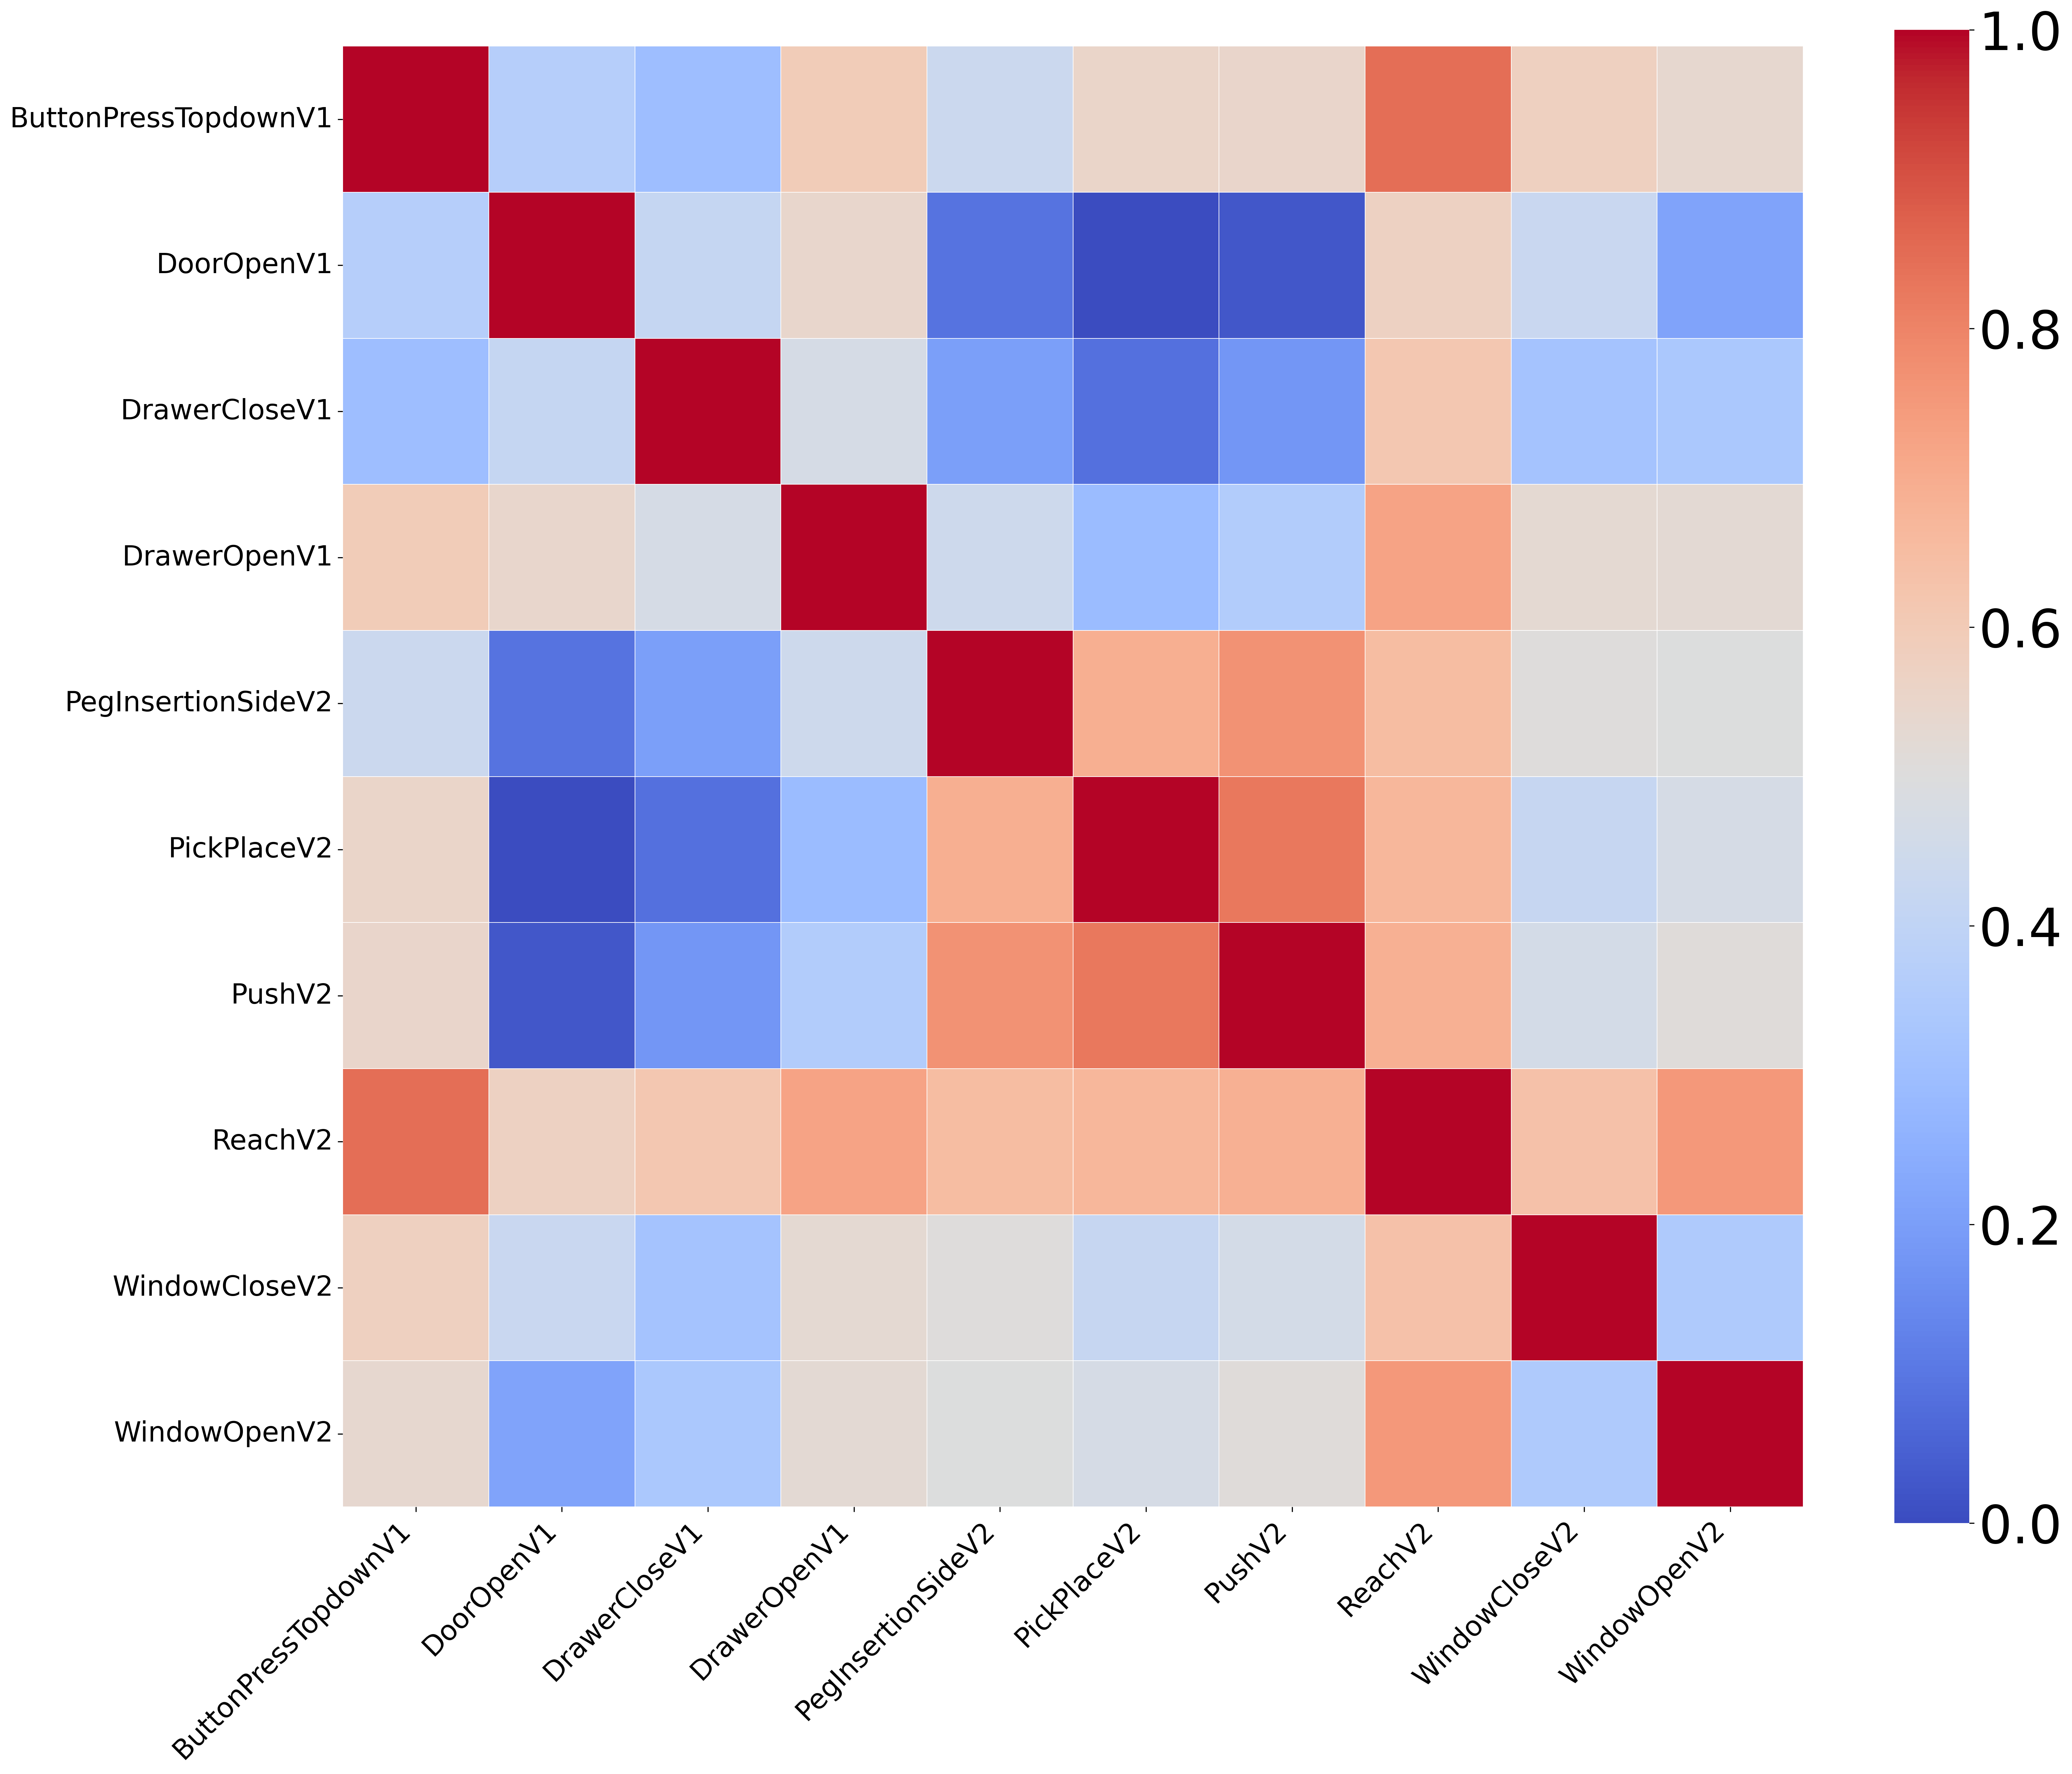
\includegraphics[width=0.48\textwidth]{task_similarity-2.png}
%     }
%     \hfill % <--- 关键：填充中间空白，把两张图挤到两边
%     % 第二个子图 (注意：这里千万不要留空行)
%     \subfigure{
%         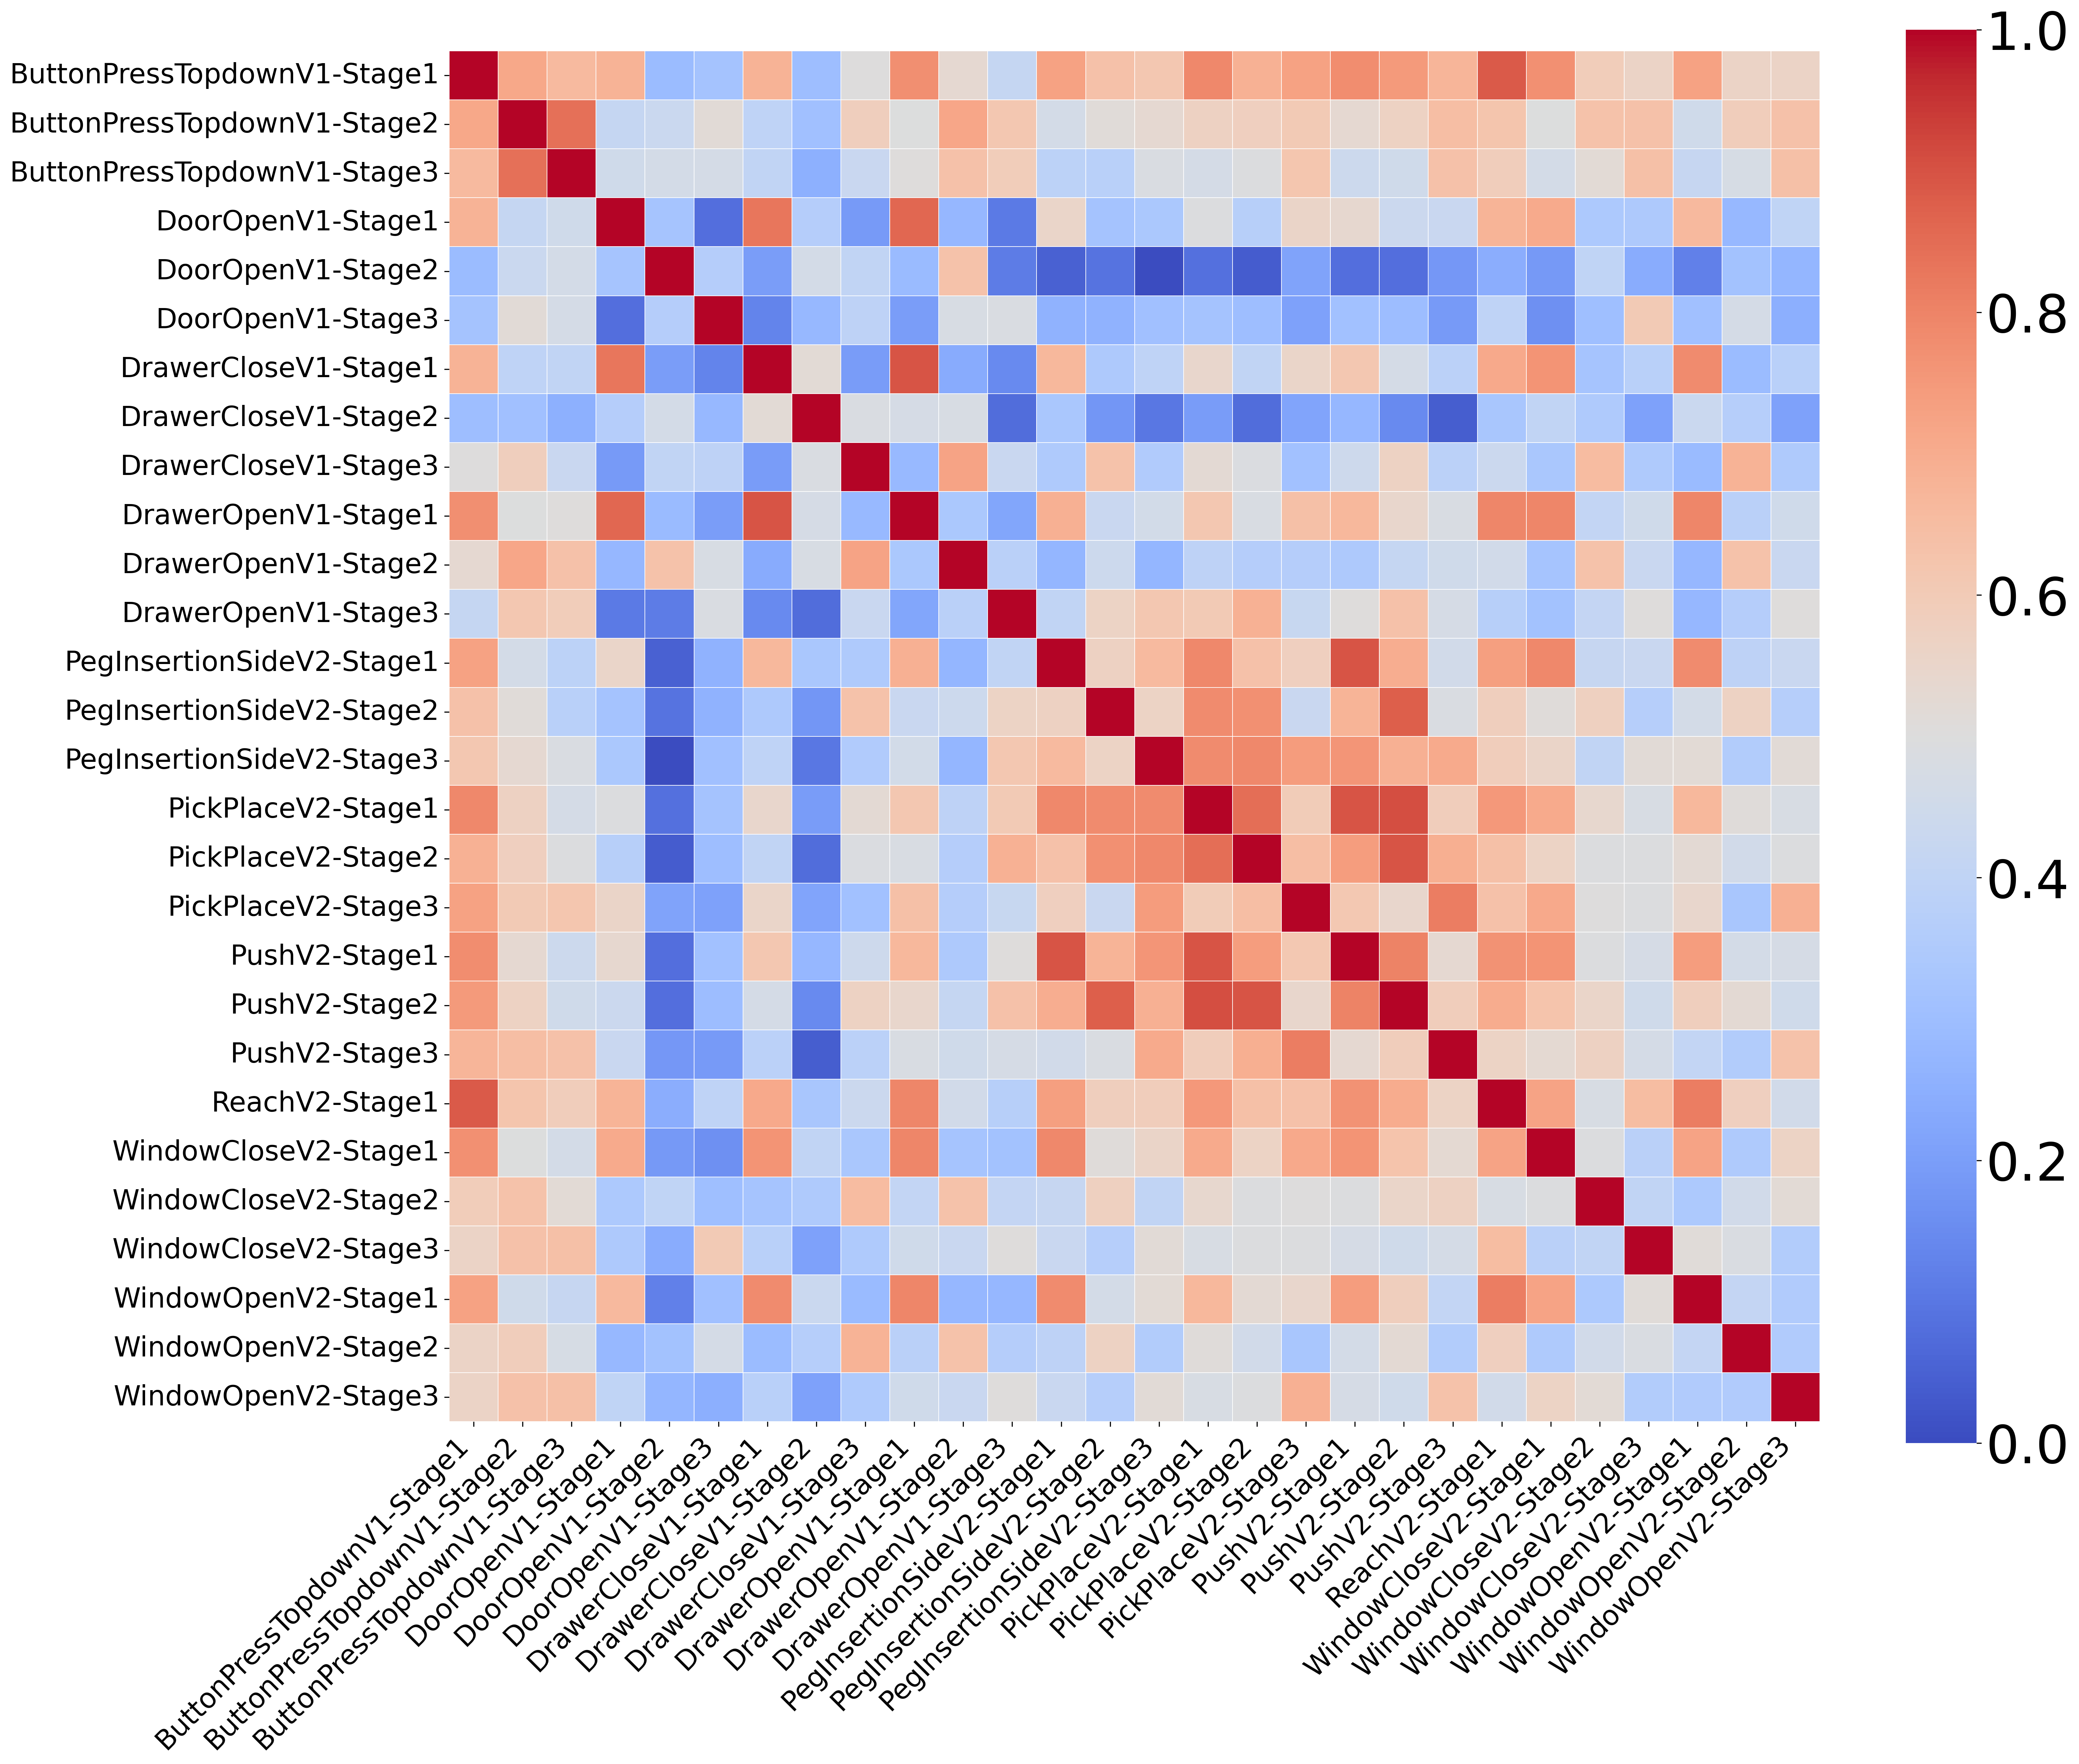
\includegraphics[width=0.48\textwidth]{stage_similarity-2.png}
%     }
    
%     \caption{MT-10 task \& stage similarity heatmap}
%     \label{fig:sim}
% \end{figure}


% \noindent\textbf{Instantiation.} 
% In our experimental environment, the general components are instantiated as follows:

% The state $s \in \mathcal{S}$ is a vector $s = (\bm{p}, \bm{o}_1, \dots, \bm{o}_{K-1}) \in \mathbb{R}^{3K}$, where $\bm{p}, \bm{o}_k$ are the 3D positions of the gripper and object. 

% The action $a \in \mathcal{A}$ is $a = (v_x, v_y, v_z, g) \in [-1,1]^4$, which controls the direction of motion of the end-effector and the magnitude of the grip.

% The reward function $\mathcal{R}^{(i)}$ is designed to follow two different paradigms: dense reward  and sparse reward. 
% In the sparse reward configuration, the agent receives no rewards other than those received upon successful steps during execution.


% Furthermore, we provide formalized descriptions of selected tasks within the widely adopted MetaWorld benchmark environment, thereby facilitating a more comprehensive understanding of stage segmentation for the reader. 
% Taking the Pick Place task as a representative example, its structure enables a decomposition into three distinct stages, each characterized by logical predicates. 
% Each stage is associated with a specific objective, and transitions between stages are determined based on state information.


% \begin{figure*}[ht]
% \centering
% \begin{minipage}{0.95\textwidth}
% {\Large\textbf{Pick Place}}

% Hand pos: $\mathbf{h}$ 

% Object pos: $\mathbf{o}$ 

% Goal pos: $\mathbf{g}$ 

% \textbf{Stage 1: MoveTo} 

% Reward function: 
% \[
% r_1 = -\|\mathbf{o} - \mathbf{h}\|
% \]

% Stage Termination condition: $\|\mathbf{o}_{xy} - \mathbf{h}_{xy}\| < \beta_1$ 

% \textbf{Stage 2: Pick \& MoveTo } 

% Reward function: 
% \[
% r_2 = -\|\mathbf{o} - \mathbf{h}\| + r_p
% \]
% \[
% r_p = 
% \begin{cases}
% 100 \cdot (o^{init}_z + \epsilon_1)  & \text{if } (o_z  - o^{init}_z) \geq \epsilon_1  \\
% 100 \cdot \min(o^{init}_z + \epsilon_1,o_z) , & \text{if } \|\mathbf{o} - \mathbf{h}\| < \beta_2 \wedge (o_z  - o^{init}_z) \geq \epsilon_2\\
% 0, & \text{otherwise}
% \end{cases}
% \]

% Stage Termination condition: $\|\mathbf{o}_z - \mathbf{h}_z\| < \beta_2$ 

% \textbf{Stage 3: PlaceObj}

% Reward function:
% \[
% r_3 = 
% \begin{cases}
% 1000 \cdot (\text{maxDist} - \|\mathbf{o} - \mathbf{g}\|) + 1000 \cdot \left( \exp\left( -\frac{(\|\mathbf{o} - \mathbf{g}\|)^2}{0.01} \right) + \exp\left( -\frac{(\|\mathbf{o} - \mathbf{g}\|)^2}{0.001} \right) \right), & \text{if} \|\mathbf{o} - \mathbf{h}\| <   \beta_3  \\
% 0, & \text{otherwise}
% \end{cases}
% \]

% Task Termination condition: $\|\mathbf{o} - \mathbf{g}\| < \beta_4$
% \end{minipage}
% \label{fig:pickplace_reward}
% \end{figure*}

% In particular, regarding the reward mechanism, the rewards employed in our experiments correspond to the reward functions prescribed by the MetaWorld environment. Notably, these functions are intricately designed and have undergone multiple iterations, underscoring the significant complexity involved. This observation substantiates that reward engineering is a domain requiring substantial expertise and extensive experimentation. Consequently, it highlights the practical necessity of multi-task learning approaches for scenarios characterized by sparse rewards.



% \subsection{B.Experiments}
% The experiments were conducted in a virtual environment running Ubuntu 20.04. The software stack includes Python 3.8, PyTorch 1.8.1, CUDA 12.2, MuJoCo 200, mujoco-py 2.0.2.8, and MetaWorld commit \#348. The hardware environment comprises a server equipped with an Intel(R) Xeon(R) Gold 5218R @ 2.10GHz CPU, four NVIDIA RTX 3090 GPUs, and 64GB of system memory.


% These baselines span major MTRL paradigms: hard parameter sharing (MT-SAC), modular routing (Soft.M), prior of natural language (CARE), architectural sharing (PTSL), and mask-based sharing (PaCo).  
% All models are implemented under comparable architectures and parameter budgets. For methods with predefined components (e.g., CARE's expert number, PaCo's mask size), we follow official design choices to ensure a fair and reproducible comparison.

% To ensure fairness, all models are implemented with comparable network architectures and hyperparameters. MT-SAC adopts the default 3-layer SAC (1.68M parameters), while CARE and PTSL retain their original expert/module structures (1.87M). PaCo employs task-specific recombination, resulting in a larger parameter count (1.68M$\times$5). For parameter efficiency analysis, we further scale all methods to 1.39M and 0.67M via width compression.


% \subsubsection{B.1  Few-shot}

% To evaluate the few-shot adaptability of SMP, we introduce two previously unseen tasks—\textit{drawer-open} and \textit{window-open} after 800k training steps. 
% As shown in Table g, SMP adapts quickly, achieving success rates of 31.6\% and 2.3\% within 300 episodes after the task is added, while MT-SAC and CARE stagnate at close to zero.
% This highlights SMP’s few-shot generalization and robustness to distributional shifts.
% SMP’s modular mask mechanism confines gradient updates to stage-relevant subnetworks, reducing interference and catastrophic forgetting. 
% This localized adaptation promotes efficient credit assignment for newly added tasks without disrupting prior knowledge.

% \begin{table}[htbp]
%   \centering
%   \caption{MT-10 Success Rate Few-Shot}
%   \label{table:g}
%   \begin{small}
%   \begin{tabular}{|c|cccc|}
%     \hline
%       \multirow{2}{*}{\textbf{Methods}} & 
%       \multicolumn{4}{c|}{\textbf{Success Rate(\%)}} \\
%       \cline{2-5}
%       & \multicolumn{1}{c}{Pre T4} & \multicolumn{1}{c}{Post T4} & \multicolumn{1}{c}{Pre T8}& \multicolumn{1}{c|}{Post T8} \\
%     \hline
%     MT-SAC     & 6.0 & 5.0 & 0.0 & 0.0  \\
%     Soft.M        & 0.0 & 0.0 & 0.0 & 0.0  \\
%     CARE       & 5.3 & 4.0 & 0.0 & 0.0  \\
%     PTSL       & 0.0 & 0.0 & 0.0 & 0.0  \\
%     PaCo       & 0.0 & 0.0 & 0.0 & 0.0  \\
%     SMP (Ours) & 3.3 & \textbf{31.6} & 0.0 & \textbf{2.3} \\
%     \hline
%   \end{tabular}
%   \end{small}
%   \label{table:g}
% \begin{quote}
% \begin{footnotesize}
% \textbf{T4, T8} = Tasks 4 and 8, introduced at 800k steps; "Pre" and "Post" refer to evaluations immediately before and after task addition.  
% All success rates are averaged over exactly 300 evaluation episodes for each phase.
% \end{footnotesize}
% \end{quote}
% \end{table}



% \subsubsection{B.2  Module ablation}

% Although our methodology features closely integrated interactions among its constituent modules, we are able to empirically isolate the effect of similarity by restricting mask sharing. As depicted in Fig.~\ref{fig:SL}, our experiments demonstrate that, while both approaches eventually converge to comparable performance levels (80.0\% after one million steps), frameworks lacking similarity guidance exhibit notably lower learning efficiency compared to those utilizing similarity-based mechanisms. This experiment provides compelling evidence that stage-wise similarity-driven knowledge transfer can significantly enhance the learning efficiency of algorithms throughout the training process.


% \begin{figure}[htbp]
%    \centering
%         \includegraphics[width=0.48\textwidth]{S-L.png} 
% \caption{Whether to use similarity knowledge sharing comparison.}
% \label{fig:SL}
% \end{figure}


% As discussed in the main text, our stage segmentation module and similarity computation module can, in principle, be replaced by alternative methodologies. For instance, given a predetermined number of stages, stage segmentation may be accomplished using attention mechanisms or Phase Learning Algorithms (PLA) applied to action data, while similarity computation can employ Dynamic Time Warping (DTW) or cross-attention mechanisms in lieu of the current Temporal Convolutional Network (TCN).

% Fig.~\ref{fig:mod} presents the results of experiments involving such module substitutions. Specifically, SMP-PLA-DTW and SMP-Att-DTW refer to frameworks in which stage segmentation is performed via PLA or multi-head attention mechanisms, and similarity computation is conducted using DTW. These approaches encounter considerable challenges in accurately segmenting stages, a difficulty that is particularly pronounced in complex robotic manipulation tasks involving intricate action sequences. Moreover, in the early phases of multi-task learning, numerous tasks fail to progress from stage one to stage two, thereby exacerbating the difficulties associated with stage demarcation and recognition. Inaccurate stage segmentation, in turn, impairs transfer precision and may even adversely affect overall performance.

% Building on these observations, we elected to use state $s$ as the criterion for stage segmentation and developed corresponding models. 
% The frameworks SMP-S-(DTW/CAtt) implement similarity computation via DTW or cross-attention mechanisms, contingent upon stage segmentation based on state information. 
% Notably, cross-attention mechanisms demonstrated relatively inferior performance, likely due to their emphasis on capturing local correlations.
% The complexity of action sequences renders such models susceptible to noise and misaligned stages during aggregation.
% DTW achieved a success rate of 78.3\%, but its adjustment based on success rate proved challenging, and its computational complexity remains prohibitively high.

% As illustrated, our preliminary experiments and subsequent ablation studies indicate that the simultaneous optimization of stage segmentation and similarity computation introduces conflicting objectives, which impedes algorithmic convergence and undermines the accuracy of stage modeling. 
% As a result, the success rate, interpretability, and stability of the stage segmentation modules did not meet expectations. Additionally, certain methods struggle to handle variable-length stage sequence data.

% To address these limitations, we adopted a rule-based stage segmentation scheme and employed Temporal Convolutional Networks (TCNs) for similarity computation. TCNs are able to effectively align stage sequences and produce fixed-length embeddings, thereby better substantiating our hypothesis. 
% We anticipate further in-depth exploration of these alternatives in future work.


% \begin{figure}[htbp]
%    \centering
%         \includegraphics[width=0.48\textwidth]{A-L.png} 
% \caption{Module replacement comparison.}
% \label{fig:mod}
% \end{figure}


% Admittedly, our current transfer strategy may not be optimally efficient. We anticipate that future work, leveraging approaches such as meta-learning, could further enhance transfer efficiency and yield superior transfer performance.



% \subsubsection{B.3  Experimental analysis}

% In terms of parameter count, the baseline MT-SAC algorithm utilizes a 3×400 network architecture, consistent with parameter configurations commonly adopted in prior literature. 
% Our proposed SMP method maintains a comparable parameter count of approximately 1.68 million, with the addition of mask-related modules and the TCN similarity module contributing only around 3,900 parameters—a negligible increase in comparison. 
% By contrast, PaCo employs multiple parameter groups for linear combination, resulting in a total parameter count of approximately 1.68 million × 5. Overall, our algorithm achieves the best performance under equivalent model sizes, demonstrating superior parameter efficiency compared to alternative approaches.


% Furthermore, by abstracting and modularizing stage segmentation, similarity computation, and mask strategy activation, our approach is compatible with a broad range of algorithms. As demonstrated in the experimental section of the main text, the CARE algorithm incorporates natural language encoding into the state $s$, thereby enhancing its ability to capture inter-task relationships. 
% CARE, when combined with SMP, achieves significant improvements on both MT-10 and MT-50 benchmarks. Specifically, on MT-10, CARE’s performance increases from 75\% to 95\%, while on MT-50, it improves from 42\% to 60\%. 
% Moreover, SMP can benefit from CARE’s state encoding, acquiring richer information and inter-task relationships, which in turn facilitates more effective training of stage strategies. 
% This synergistic integration can be extended to other MTRL methods that utilize state encoding or representation learning.


% \subsection{C.Code}

% %\textbf{The source code and datasets are anonymously available at }{https://anonymous.4open.science/r/SMP-6644/}

% \textbf{The source code and datasets are included as part of the anonymous Supplementary Material accompanying this submission.}

% We designed and systematically evaluated the hyperparameters for our proposed SMP framework through extensive preliminary experiments tailored to the specific task requirements.
% For baseline methods, we closely followed the original papers and official implementations to replicate their results, aligning all key hyperparameters to ensure fair and reproducible comparisons.

% \textbf{SMP:} 

% Pruning ratio: 0.2; 

% Evaluation interval $B$: Currently set to 6000. This parameter regulates the frequency of SMP usage and updates, and periodically clears the repository of optimal behavior sequences to prevent anomalies arising from reward assessment discrepancies at different time intervals. A value in the range of 3000–12000 is generally appropriate.
% Evaluation period $L$: Currently set to 600. This parameter controls the update frequency, thereby managing computational resource usage and preventing excessive time consumption. It can be set to any value between the maximum number of steps per episode and $B$.

% Similarity threshold($\mathcal{S}_{\text{thresh}}$): As we select the stage with the highest similarity for knowledge sharing, this threshold can be understood as being automatically adjusted based on environment and task diversity. 
% Generally, it is set to 0.0, but for tasks with greater disparity, values around 0.5 may be used.

% Success rate threshold($suc_{\text{thresh}}$): 0.7. The rationale for this setting is that, upon successful learning, the single-task success rate can typically be maintained above 0.7, which can be interpreted as convergence of the stage strategy. (If this is difficult to set, it may be gradually increased to around 0.8 based on SAC entropy changes or training steps.)

% TCN parameters are as follows: channels={$[8, 16, 16]$}; kernel\_size=3; embedding\_dim=32.

% \textbf{Baseline parameters:} 

% SAC: $\gamma=0.99$; init\_temperature=0.01; optimizer: Adam.

% CARE: Number of MoE components: 4.

% PTSL: Projection layer size: MT-10: pal\_dim=50; MT-50: pal\_dim=32.

% PaCo: Number of parameter groups: 5.


% \subsection{D.Pseudocode}

% \begin{algorithm}[H]
% \caption{Stage-Masked Policy(SMP)}
% \label{alg:sa-aps}
% \begin{algorithmic}[1] % Enable line numbers
%     \STATE \textbf{Input}: Task set $\mathcal{T}$, environment $\mathcal{E}$, total steps $N$, evaluation interval $B$,evaluation period $L$
%     \STATE \textbf{Initialize}: policy parameters $\theta$, critic parameters $\phi_1, \phi_2$, target networks $\phi_1', \phi_2'$
%     \STATE Initialize stage masks $M_{k}^{(i,l)}$ similarity matrix $\mathcal{S}$, similarity model $\mathcal{M}_{\text{sim}}$, and optimal sequence buffer $\mathbb{A}^*$
%     \STATE Initialize experience replay buffer $\mathcal{D}$
%     \WHILE{step $< N$}
%         \FOR{each task $T^{(i)} \in \mathcal{T}$}
%             \STATE Observe state $\bm{s}_j$, determine stage $k_j = \Psi(\bm{s}_{t}, T^{(i)})$
%             \STATE Select action $\bm{a}_{t} \sim \pi_\theta(\cdot \mid \bm{s}_{t}, T^{(i)}, M^{(i)}_{k_{t}})$
%             \STATE Execute $\bm{a}_{t}$, collect reward $R_i$, next state $\bm{s}'_{t}$, done flag
%             \STATE Store transition $(\bm{s}_{t}, \bm{a}_{t}, R^{(i)}, \bm{s}'_{t}, T^{(i)}, k_{t})$ in $\mathcal{D}$
%         \ENDFOR
%         \STATE Sample batch $\mathcal{B}$ from $\mathcal{D}$ and perform SAC update on $\theta$, $\phi_1$, $\phi_2$, $\alpha^{(i)}$
%         \IF{step $\% B == 0 $}
%             \STATE  Eval step $=1$ to $L$
%             \FOR{$\text{Eval step}<L$ each task $T^{(i)}$}
%                 \STATE Collect full trajectories and update best action sequence buffer $\mathbb{A}^*$
%                 \STATE Compute success rate $suc^{(i)}$ and stage-level performance change $\Delta suc^{(i)}$
%                 \FOR{each active stage $(T^{(i)}, k)$}
%                     \STATE Estimate importance $I^{(l)}$ from gradients $\left| \frac{\partial \mathcal{L}_\pi}{\partial \theta^{(l)}} \right|$
%                     \STATE Prune low-importance neurons using $p_{\text{prune}}(i)$
%                     \STATE Regrow masked neurons using $p_{\text{regrow}}(i)$
%                 \ENDFOR
%             \ENDFOR
%             \FOR{each stage pair $((T^{(i)}, k_a), (T^{(j)}, k_b))$}
%                 \STATE Compute $\mathcal{K}^{(i,j)}_{(a, b)} = \mathcal{M}_{\text{sim}}(seq_a, seq_b; \omega)$
%                 \STATE Update $\mathcal{M}_{\text{sim}}$ via MSE loss $\mathcal{L}_{\text{sim}}$
%             \ENDFOR
%             \FOR{each task-stage $(T^{(i)}, a)$}
%             \STATE $(T^{(j)}, b) \gets$ {Highest similarity}$(T^{(i)}, a)$
%             \IF{$\mathcal{K}^{(i,j)}_{(a, b)} > \mathcal{S}_{\text{thresh}} \& suc^{(j)}_s > suc_{\text{thresh}}$ }
%              \STATE Update $M_{a}^{(i,l)}$ from $M_{b}^{(j,l)}$ probabilistically using $P_{\text{update}}$
%             \ENDIF
%         \STATE  Eval step $+1$
%         \ENDFOR
%         \ENDIF
%     \ENDWHILE
% \end{algorithmic}
% \label{alg:sa-aps}
% \end{algorithm}



\end{document}
